\documentclass[10pt]{article}

\usepackage[letterpaper,margin=0.85in]{geometry}
\usepackage[T1]{fontenc}
\usepackage[utf8]{inputenc}
\usepackage{lmodern}
\usepackage{microtype}
\usepackage{amsmath,amssymb}
\usepackage{booktabs}
\usepackage{array}
\usepackage{enumitem}
\usepackage{xcolor}
\usepackage{tikz}
\usetikzlibrary{arrows.meta,positioning,fit,calc,shapes.geometric}
\usepackage{hyperref}
\usepackage[numbers,sort&compress]{natbib}

\definecolor{navy}{HTML}{17365D}
\definecolor{blue}{HTML}{2F75B5}
\definecolor{pale}{HTML}{EAF2F8}
\definecolor{green}{HTML}{E2F0D9}
\definecolor{orange}{HTML}{FCE4D6}
\hypersetup{colorlinks=true,linkcolor=navy,citecolor=blue,urlcolor=blue}
\setlist{nosep,leftmargin=*}
\setlength{\emergencystretch}{3em}
\newcolumntype{P}[1]{>{\raggedright\arraybackslash}p{#1}}
\newcommand{\method}{\textsc{Context2Card}}
\newcommand{\silent}{\texttt{stay\_silent}}
\newcommand{\serve}{\texttt{serve}}
\newcommand{\needrecord}{\texttt{need\_record}}
\newcommand{\card}{\texttt{card}}

\title{Context-to-Card: A Scenario-Centered Framework for\\
Context-Aware Agent Services}
\author{Anonymous Authors}
\date{}

\begin{document}
\maketitle

\begin{abstract}
Proactive agent services face a decision that ordinary recommendation systems often leave implicit: whether a service should be offered to a particular user at this particular moment. A large set of user, temporal, environmental, event, and place signals does not by itself define a useful service. Directly passing all signals to a text generator can produce content that is weakly related, stale, unsupported, or unnecessarily interruptive. We present \method{}, a scenario-centered framework that makes the intermediate reasoning contract explicit. The framework translates structured Context into a bounded situation hypothesis and a latent-need record, performs candidate and fact checks, chooses between a service and an explicit silence outcome, and only then generates a card. We instantiate two card types: an event alert card anchored by a current Event, and a point-of-interest (POI) card that constructs a need before filtering and ranking nearby candidates. Positive and negative synthetic cases are accompanied by a shared rubric covering contextual fit, user value, factual grounding, readability, and restraint. We release a dependency-free reference implementation, schemas, 40 synthetic cases, validators, and an interactive static demo. The released implementation is a transparent research baseline rather than evidence of production or online effectiveness; this distinction is made explicit throughout the paper.
\end{abstract}

\section{Introduction}

Recommendation becomes a different problem when the system is allowed to interrupt a user. A conventional recommender can optimize relevance among items. A proactive card service must additionally decide whether the present situation warrants service, whether the facts are still actionable, and whether the output can be traced to evidence. Location and time are known to be important contextual dimensions in recommender systems \citep{adomavicius2011context}; however, simply adding more context fields does not explain how an agent should move from observations to a service decision.

We study the following problem. Given a structured Context $C$, a card type $k$, and (for POI cards) a candidate set $P$, produce either a card or a justified silence:
\begin{equation}
  f(C,k,P) \rightarrow (d, r, y), \qquad d \in \{\serve,\silent\},
\end{equation}
where $r$ is an auditable need record and $y$ is card content when $d=\serve$. The goal is not to maximize the number of cards. It is to make the service decision and the generated content appropriate to the current situation, useful for the user, grounded in available facts, and reproducible for evaluation.

\paragraph{Contributions.}
This paper makes four practical contributions:
\begin{enumerate}
  \item We define a scenario-centered pipeline in which Context is translated into an auditable \needrecord{} before candidate selection or language generation.
  \item We provide two distinct decision contracts: an Event-anchored alert path and a need-first POI path, while sharing a common service-decision and evaluation layer.
  \item We treat \serve{} and \silent{} as symmetric outputs and provide positive and negative synthetic cases for both card types.
  \item We release a transparent reference implementation, schemas, data, validators, and a static demo that expose intermediate outputs rather than only final text.
\end{enumerate}

The release deliberately does not claim improved click-through, user satisfaction, or real-world recommendation quality. Its purpose is to make the reasoning structure and evaluation surface inspectable and replaceable.

\begin{table}[t]
\centering
\small
\caption{Claims supported by the public release and claims deliberately left open.}
\label{tab:claims}
\begin{tabular}{P{0.28\linewidth}P{0.31\linewidth}P{0.28\linewidth}}
\toprule
Claim & Evidence included in the release & Not established by this release \\
\midrule
Auditable need interface & Formal record, schemas, inspectable runtime output & Semantic correctness of inferred needs \\
Two card contracts & Separate Event and POI paths in code and Cases & Superiority to a recommender or agent baseline \\
Abstention wiring & Negative Cases and one-factor gate mutations & Calibrated risk--coverage or interruption utility \\
Grounded copy protocol & Rubric and evidence-before-expression rule & Human-rated value, naturalness, or persuasion \\
\bottomrule
\end{tabular}
\end{table}

\section{Related Work}

\paragraph{Context-aware recommendation.}
Context-aware recommender systems incorporate dimensions such as time, location, and social context into recommendation models \citep{adomavicius2011context}. The classic pre-filtering, post-filtering, and contextual-modeling perspectives motivate our separation of hard constraints from matching signals. Our focus is complementary: we make the intermediate scenario and service decision explicit for proactive cards, including the option not to recommend.

Mobile recommendation work has also combined location, activity, and implicit intent to rank places and entities on the go \citep{zhuang2011mobile}. We retain that emphasis on current context, but make the latent need and the serve-or-silence decision inspectable before a place is ranked.

\paragraph{Agent reasoning and acting.}
ReAct interleaves reasoning traces and actions to improve interaction with external sources and exception handling \citep{yao2023react}. Generative Agents use observations, memory, reflection, and planning to produce believable behavior \citep{park2023generative}. We do not attempt to reproduce their general agent capabilities. Instead, we use a small, bounded record that exposes only the evidence and constraints needed for a card-service decision.

\paragraph{Explainability and evaluation.}
Explainable recommendation research distinguishes user-facing explanations from explanations for system designers and studies their effect on transparency and trust \citep{zhang2018explainable,chen2022measuring}. Our output contract separates short card copy from internal reasons and evidence. Offline evaluation is useful but imperfect for interactive recommenders \citep{aouali2022offline,hidasi2023flaws}; consequently, our synthetic results are reported as reproducibility checks, not as estimates of online utility.

Selective prediction formalizes the option to reject uncertain inputs instead of forcing a prediction \citep{geifman2019selectivenet}; recommender simulators such as RecSim separate generated environments, user choice, and agent policy for sequential evaluation \citep{ie2019recsim}. These works motivate our abstention objective and our explicit statement that the current release is static and rule-derived rather than calibrated or interactive.

\begin{table}[t]
\centering
\small
\caption{Positioning against two closest methodological precedents.}
\label{tab:related-positioning}
\begin{tabular}{P{0.22\linewidth}P{0.32\linewidth}P{0.34\linewidth}}
\toprule
Work & What it makes explicit & Difference in \method{} \\
\midrule
Woerndl et al.~\citep{woerndl2011proactivity} & Separates when a mobile recommendation should be proactive from which item to recommend & Adds a bounded need record, two card-specific contracts, symmetric silence, and a public synthetic artifact \\
RecMind~\citep{wang2024recmind} & Uses an LLM agent with planning and external recommendation tools & Provides an agent-compatible contract without requiring an LLM; the released implementation is deterministic and exposes evidence and gates \\
\bottomrule
\end{tabular}
\end{table}

The comparison is deliberately narrow. Context-aware modeling, mobile location recommendation, selective prediction, simulation, and explainability provide supporting foundations, but this paper does not claim to replace those model families. Its contribution is the inspectable service contract that connects them to an interruptive card decision.

\section{Problem Formulation and Design Principles}

Let $C=(U,E,V,X)$ contain user features $U$, environment features $E$, an optional Event $V$, and an optional POI candidate set $X$. The framework first constructs a situation hypothesis $s$ and a need record $r$:
\begin{equation}
  (s,r)=g(C,k), \qquad
  r=(\text{situation},\text{need},\text{constraints},\text{evidence},\text{confidence}).
\end{equation}
The service decision is then computed from the record and relevant facts:
\begin{equation}
  d=h(r,V,X).
\end{equation}
Only if $d=\serve$ is card generation invoked:
\begin{equation}
  y=q(r,V,X,k).
\end{equation}

The decision can be interpreted as a selective-service objective rather than a maximization of card volume. Let $B(C)$ denote expected user benefit, $I(C)$ interruption cost, $R(C)$ unsupported-claim risk, and $F(C)$ action friction. A production policy may serve only when hard constraints pass and
\begin{equation}
  U(\serve\mid C)=B(C)-\lambda I(C)-\mu R(C)-\nu F(C)>0.
\end{equation}
The public implementation does not estimate these terms or claim calibrated utility; it uses transparent demonstration thresholds. The equation makes explicit which quantities a future risk--coverage or user study would need to measure.

The separation imposes five design principles:
\begin{enumerate}
  \item \textbf{Evidence before expression:} user-visible claims must be supported by fields in the Case.
  \item \textbf{Situation before candidate:} a POI is selected to satisfy a translated need, not to justify a preselected item.
  \item \textbf{Decision before generation:} generation cannot turn a failed service check into a card.
  \item \textbf{Silence is a result:} no-card outcomes carry a reason and are included in evaluation.
  \item \textbf{Replaceable modules:} retrieval, ranking, and generation can be replaced without removing the intermediate contract.
\end{enumerate}

\section{Framework Architecture}

Figure~\ref{fig:architecture} shows the complete data flow. The dashed boundary separates the context-to-card method from the final presentation surface.

\begin{figure}[t]
\centering
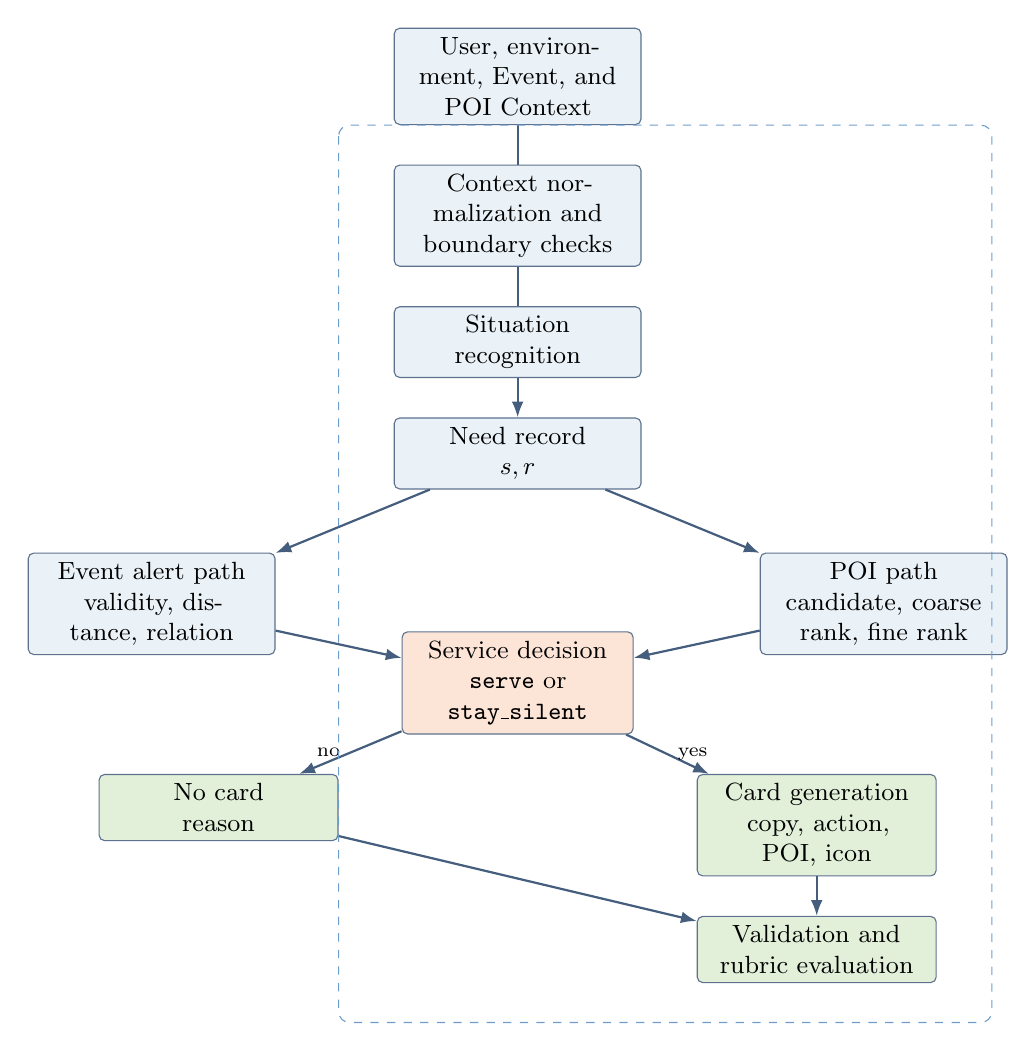
\begin{tikzpicture}[
  node distance=5mm and 8mm,
  box/.style={draw=navy!70,rounded corners=2pt,fill=pale,align=center,minimum height=8mm,text width=29mm,font=\small},
  decision/.style={draw=navy!70,rounded corners=2pt,fill=orange,align=center,minimum height=8mm,text width=27mm,font=\small},
  outbox/.style={draw=navy!70,rounded corners=2pt,fill=green,align=center,minimum height=8mm,text width=28mm,font=\small},
  arr/.style={-{Latex[length=2mm]},thick,draw=navy!80}
]
\node[box] (input) {User, environment, Event, and POI Context};
\node[box,below=of input] (norm) {Context normalization and boundary checks};
\node[box,below=of norm] (scene) {Situation recognition};
\node[box,below=of scene] (need) {Need record\\$s,r$};
\node[box,below left=8mm and 15mm of need] (event) {Event alert path\\validity, distance, relation};
\node[box,below right=8mm and 15mm of need] (poi) {POI path\\candidate, coarse rank, fine rank};
\node[decision,below=18mm of need] (dec) {Service decision\\$\serve$ or $\silent$};
\node[outbox,below left=of dec] (silent) {No card\\reason};
\node[outbox,below right=of dec] (gen) {Card generation\\copy, action, POI, icon};
\node[outbox,below=of gen] (eval) {Validation and rubric evaluation};
\draw[arr] (input)--(norm)--(scene)--(need);
\draw[arr] (need)--(event);
\draw[arr] (need)--(poi);
\draw[arr] (event)--(dec);
\draw[arr] (poi)--(dec);
\draw[arr] (dec)--node[left,font=\scriptsize]{no}(silent);
\draw[arr] (dec)--node[right,font=\scriptsize]{yes}(gen);
\draw[arr] (gen)--(eval);
\draw[arr] (silent)--(eval);
\draw[dashed,rounded corners,draw=blue!70] ($(norm.north west)+(-7mm,5mm)$) rectangle ($(eval.south east)+(7mm,-5mm)$);
\end{tikzpicture}
\caption{The Context-to-Card architecture. Light nodes are transformations, orange nodes are service gates, green nodes are externally visible or evaluable outputs, and the dashed boundary marks the shared method. The need record is the explicit interface between context interpretation and service execution.}
\label{fig:architecture}
\end{figure}

\subsection{Context roles}

Every field is assigned a role before use:
\begin{itemize}
  \item \textbf{Evidence} directly describes a fact, such as an active Event or an open POI.
  \item \textbf{Relation signal} describes why the fact may matter to this user, such as a preference overlap or relevance score.
  \item \textbf{Constraint} limits what can be served, such as distance, time window, weather exposure, or availability.
\end{itemize}
The same field must not be treated as a universal positive signal. A preference can establish a relation but cannot alone prove an immediate intention to act.

\begin{table}[t]
\centering
\small
\caption{Alignment between the public reference baseline and the broader production protocol.}
\label{tab:alignment}
\begin{tabular}{P{0.22\linewidth}P{0.34\linewidth}P{0.31\linewidth}}
\toprule
Module & Implemented in the public baseline & Production extension point \\
\midrule
Summary & Binary \texttt{summary\_theme} match contributes to POI score & Semantic Summary matching and calibrated confidence \\
Event compatibility & Status, distance, and relevance gates & Detailed time-window, weather-exposure, Action, and target checks \\
POI quantity & Top 3 after score and distance sort & Independent multi-POI topic-coherence and diversity filter \\
Provenance & Human-readable evidence strings & Field-path references and machine-checkable constraint results \\
Language generation & Deterministic templates for reproducibility & Replaceable generator with copy-policy and linguistic validation \\
\bottomrule
\end{tabular}
\end{table}

\subsection{The need record as a bounded interface}

The need record is intentionally small. It contains a situation statement, a latent need, explicit constraints, supporting evidence, and a confidence value. It is not a user-facing explanation and it is not a free-form chain-of-thought. Downstream components may use only needs and constraints supported by the record. This limits unsupported inference and makes errors localizable.

\section{Two Operational Views}

The method has a data-construction view and a runtime view (Figure~\ref{fig:views}). Confusing them creates unrealistic cases: a dataset builder can inspect a global Event or POI table, whereas a runtime component must use only the fields present in the Case.

\begin{figure}[t]
\centering
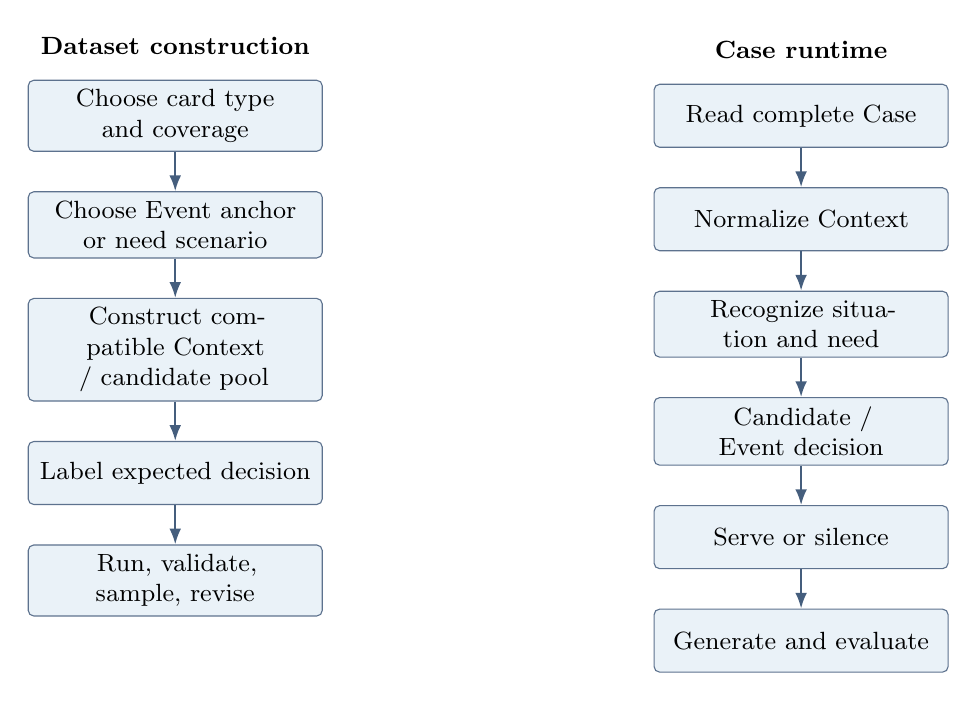
\begin{tikzpicture}[
  node distance=5mm and 12mm,
  box/.style={draw=navy!70,rounded corners=2pt,fill=pale,align=center,minimum height=8mm,text width=35mm,font=\small},
  arr/.style={-{Latex[length=2mm]},thick,draw=navy!80}
]
\node[box] (a1) {Choose card type and coverage};
\node[box,below=of a1] (a2) {Choose Event anchor or need scenario};
\node[box,below=of a2] (a3) {Construct compatible Context / candidate pool};
\node[box,below=of a3] (a4) {Label expected decision};
\node[box,below=of a4] (a5) {Run, validate, sample, revise};
\node[box,right=42mm of a1] (b1) {Read complete Case};
\node[box,below=of b1] (b2) {Normalize Context};
\node[box,below=of b2] (b3) {Recognize situation and need};
\node[box,below=of b3] (b4) {Candidate / Event decision};
\node[box,below=of b4] (b5) {Serve or silence};
\node[box,below=of b5] (b6) {Generate and evaluate};
\foreach \u/\v in {a1/a2,a2/a3,a3/a4,a4/a5,b1/b2,b2/b3,b3/b4,b4/b5,b5/b6} {\draw[arr](\u)--(\v);}
\node[font=\small\bfseries,above=2mm of a1] {Dataset construction};
\node[font=\small\bfseries,above=2mm of b1] {Case runtime};
\end{tikzpicture}
\caption{Dataset construction and runtime are related but distinct operational views.}
\label{fig:views}
\end{figure}

\section{Event Alert Cards}

\subsection{Contract and anchor}

An Event alert card answers whether one current Event is worth surfacing now. The Event is the fact anchor. The public baseline expects a theme, status, distance, user-relevance score, factual line, executable action, and bilingual icon tag. Location-list or ranking content is not treated as an Event in this path; it belongs to the POI path.

\subsection{Scenario-construction paths}

\begin{figure}[t]
\centering
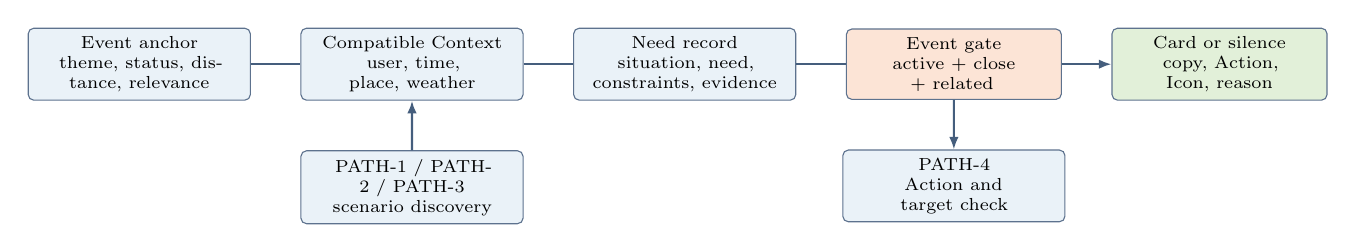
\begin{tikzpicture}[
  scale=0.90,transform shape,
  node distance=4mm and 7mm,
  box/.style={draw=navy!70,rounded corners=2pt,fill=pale,align=center,minimum height=8mm,text width=29mm,font=\scriptsize},
  gate/.style={draw=navy!70,rounded corners=2pt,fill=orange,align=center,minimum height=8mm,text width=28mm,font=\scriptsize},
  outbox/.style={draw=navy!70,rounded corners=2pt,fill=green,align=center,minimum height=8mm,text width=28mm,font=\scriptsize},
  arr/.style={-{Latex[length=1.6mm]},thick,draw=navy!80}
]
\node[box] (e1) {Event anchor\\theme, status, distance, relevance};
\node[box,right=of e1] (e2) {Compatible Context\\user, time, place, weather};
\node[box,right=of e2] (e3) {Need record\\situation, need, constraints, evidence};
\node[gate,right=of e3] (e4) {Event gate\\active + close + related};
\node[outbox,right=of e4] (e5) {Card or silence\\copy, Action, Icon, reason};
\draw[arr](e1)--(e2)--(e3)--(e4)--(e5);
\node[box,below=7mm of e2] (p) {PATH-1 / PATH-2 / PATH-3\\scenario discovery};
\node[box,below=7mm of e4] (p4) {PATH-4\\Action and target check};
\draw[arr](p)--(e2);
\draw[arr](e4)--(p4);
\end{tikzpicture}
\caption{Event alert workflow. Scenario paths discover candidate situations; the Event gate and Action check occur before content generation.}
\label{fig:event-workflow}
\end{figure}

Dataset construction can discover an alert scenario through three paths, followed by an action-compatibility check:
\begin{description}[leftmargin=3.2cm,labelwidth=2.9cm]
  \item[PATH-1 (top-down)] Start from a broad life domain, independently propose a current opportunity or change, then verify it against an allowed Event.
  \item[PATH-2 (seeded expansion)] Use an old sub-scenario only as an idea seed; reconstruct it with currently usable Context and an allowed Event. Deprecated dependencies are removed rather than mocked back into existence.
  \item[PATH-3 (bottom-up)] Combine user relation, a current signal, and an actionable fact from available Context; only then assign the result to a broad domain.
\end{description}
PATH-4 is not a scenario generator. After an alert opportunity is established, it checks whether one available Action naturally completes the service and, for a place action, whether the target POI is traceable. The public reference data does not persist a full construction trace, but the method requires the trace in a production dataset.

\subsection{Event--Context compatibility}

After selecting an Event, the data builder constructs a compatible user and environment Context. Compatibility is checked across five dimensions: time and Event window, spatial distance, user relation, weather versus indoor/outdoor exposure, and Action support. A missing compatibility fact is not silently filled at runtime; the Case is revised during dataset construction or labeled negative.

\subsection{Decision rule}

The transparent baseline serves an Event only when:
\begin{equation}
  \mathbb{1}[\text{status}=\text{active}]\land
  \mathbb{1}[\text{distance}\leq 8]\land
  \mathbb{1}[\text{relevance}\geq 0.6].
\end{equation}
Otherwise it returns \silent{} with one or more reasons. The numerical thresholds are demonstration parameters, not claims about a universal production policy.

\subsection{Content contract}

The main copy expresses user relation, present value, and the concrete Event. It is limited to 16 Chinese characters in the source product; the public English paper describes this as a bounded short string rather than imposing a language-specific character count. The sub-copy carries a factual line from the Event. One user-facing Action is emitted, using an executable verb phrase rather than an information label. The icon is selected primarily from Event or POI type, with weather as an auxiliary signal, and is emitted in English and Chinese tags. For reproducibility, the public baseline instantiates this contract with deterministic templates; it does not claim a general-purpose natural-language generator.

	\paragraph{Worked example.}
Given a local user with outdoor and low-intensity preferences, a sunny morning, and an active market 1.3 km away, the record may state: "nearby, currently active market; decide whether surfacing it now lowers discovery cost." The decision is \serve{}. The card can contain a value-oriented main copy, the factual time-and-place line as sub-copy, the Action "Go see," and the icon tag `market / market'. If the same Event is expired, the result is \silent{} even when distance and preference relation remain high.

\section{POI Recommendation Cards}

\begin{figure}[t]
\centering
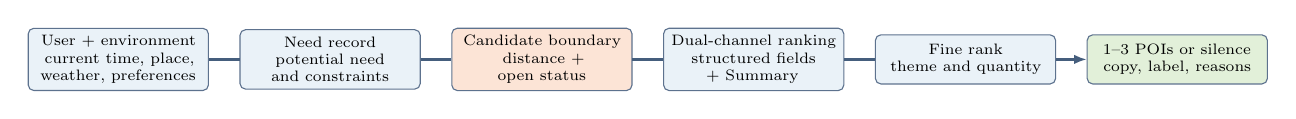
\begin{tikzpicture}[
  scale=0.78,transform shape,
  node distance=4mm and 5mm,
  box/.style={draw=navy!70,rounded corners=2pt,fill=pale,align=center,minimum height=8mm,text width=27mm,font=\scriptsize},
  gate/.style={draw=navy!70,rounded corners=2pt,fill=orange,align=center,minimum height=8mm,text width=27mm,font=\scriptsize},
  outbox/.style={draw=navy!70,rounded corners=2pt,fill=green,align=center,minimum height=8mm,text width=27mm,font=\scriptsize},
  arr/.style={-{Latex[length=1.6mm]},thick,draw=navy!80}
]
\node[box] (p1) {User + environment\\current time, place, weather, preferences};
\node[box,right=of p1] (p2) {Need record\\potential need and constraints};
\node[gate,right=of p2] (p3) {Candidate boundary\\distance + open status};
\node[box,right=of p3] (p4) {Dual-channel ranking\\structured fields + Summary};
\node[box,right=of p4] (p5) {Fine rank\\theme and quantity};
\node[outbox,right=of p5] (p6) {1--3 POIs or silence\\copy, label, reasons};
\draw[arr](p1)--(p2)--(p3)--(p4)--(p5)--(p6);
\end{tikzpicture}
\caption{POI workflow.}
\label{fig:poi-workflow}
\end{figure}

\subsection{Need-first candidate construction}

POI cards are not interest-only recommendations. They are anchored in the user's current time, place, weather, and usable profile features. The system first translates these signals into a low-decision-cost need and constraints. Distance is the first candidate boundary, followed by availability. Only within that boundary are preference, structured POI attributes, and Summary features compared.

\subsection{Candidate pool}

Let $P$ be the input candidate pool. The baseline keeps a candidate $p$ only if:
\begin{equation}
  \text{distance}(p)\leq 5\ \text{km}\quad\land\quad\text{status}(p)=\text{open}.
\end{equation}
The boundary can be changed by city, mode, time, or user state without changing the ordering principle. A candidate pool is not the final result; it is the evidence set from which the final 1--3 POIs must be selected.

\subsection{Coarse ranking with Summary and structured features}

The baseline score illustrates the intended two-channel use of POI data:
\begin{equation}
  S(p)=0.45D(p)+0.35O(p)+0.20M(p),
\end{equation}
where $D$ is a normalized distance score, $O$ is preference-tag overlap, and $M$ is a Summary-theme match. In the reference code, the Summary signal is represented by a transparent `summary\_theme` match against POI tags or user tags. More advanced systems may replace this binary feature with semantic matching, but Summary must affect candidate retention or ranking, not merely appear in a post-hoc explanation.

\subsection{Fine ranking and quantity}

Candidates are sorted by score and distance, with at most three selected. One POI is appropriate when one candidate clearly dominates; two or three are appropriate when candidates share a coherent theme and provide useful choice. The baseline returns \silent{} when there is no valid candidate or the highest score is below 0.42. The public baseline does not implement an independent topic-consistency filter; topic consistency is a method requirement and an explicit extension point.

\subsection{Content and image-label contract}

The internal theme explains why the selected POIs belong together. The main copy communicates current user value and the concrete type of outing; the sub-copy supplies one line of grounded auxiliary facts rather than a generic ETA. Internal recommendation reasons mention distance, preference overlap, Summary evidence, and structured attributes, but are not shown as user copy. A shared image label is selected with the priority "specific secondary tag, then suitable primary category." If neither applies, the output explicitly records that no suitable label was found rather than inventing a universal fallback.

\paragraph{Worked example.}
For an afternoon user who prefers outdoor, low-intensity activities, the need record can be "find an open, nearby, low-decision-cost outdoor option." Two nearby open POIs whose Summaries describe a greenway walk and an easy cycling route can share the internal theme "nearby light outdoor." A short main copy and a factual sub-copy are generated only after these POIs have been selected. A distant POI with a matching "outdoor" tag is filtered before ranking.

\section{Service Decision and Card Generation}

The decision layer is shared, while the evidence tested is card-specific:

\begin{table}[t]
\centering
\small
\caption{Decision contracts for the two card types.}
\label{tab:contracts}
\begin{tabular}{p{0.21\linewidth}p{0.32\linewidth}p{0.32\linewidth}}
\toprule
 & Event alert & POI recommendation \\
\midrule
Fact anchor & One current Event & Candidate POI set \\
Primary question & Is this Event worth surfacing now? & Which nearby POIs satisfy the current need? \\
First filters & Status, distance, relevance, time & Distance, open status, need compatibility \\
Final object & One Event, one Action, one Icon & One to three POIs, theme, copy \\
Silence examples & Expired, too far, weak relation & No valid candidate, too far, unavailable, weak match \\
\bottomrule
\end{tabular}
\end{table}

Generation is invoked only after \serve{}. The card output is separated into user-facing fields (main copy, sub-copy, Action or POI name) and internal fields (need record, evidence, theme, decision reasons). This separation allows concise presentation and detailed audit simultaneously. In the public code, ``generation'' means deterministic template rendering; a production system may replace $q$ with a constrained language model, but must preserve the evidence and length/punctuation contract.

\section{Synthetic Dataset Construction}

\subsection{Case schema}

Each Case contains a unique ID, card type, Context, and expected decision. Running a Case produces an actual decision, need record, card, reasons, and source marker. The reference release has 40 Cases: 10 positive and 10 negative for each card type. Event negatives cover expired status, excessive distance, and low relevance. POI negatives contain only closed or overly distant candidates.

\subsection{Coverage and distribution}

Coverage is defined over factors that can change a decision or output: time of day, weather, local versus visiting status, preference combinations, Event themes, POI themes, candidate distance, candidate count, ordinary versus special dates, and positive versus negative polarity. The aim is not to enumerate every Cartesian product. The public 40-Case release covers a subset of these factors (including time, weather, locality, preference combinations, themes, distance, candidate count, and polarity); special-date variation is specified by the construction protocol but is not claimed as covered by this small release. Each included factor is varied enough to expose a different reasoning boundary, while avoiding a synthetic distribution in which every Case contains a special date or a single repeated template.

\subsection{Positive and negative cases}

Positive Cases test whether the system serves when facts are current, related, actionable, and sufficiently close. Negative Cases test restraint. A negative result is not a failed generation: it is a valid service outcome with a reason. The two card types have independent negative sets; a POI card does not evade a negative condition by delegating to an Event card.

\section{Evaluation Protocol}

\subsection{Automated checks}

The reference validator checks JSON parseability, required top-level and need-record keys, card-type and decision enumerations, served-card field presence, POI cardinality, expected/actual decision agreement, null card content for silence, duplicate IDs, confidence range, and a small set of public-boundary tokens. It does not prove semantic relevance, factual provenance, Summary quality, or naturalness. Those limitations are part of the release contract.

\subsection{Rubric}

The shared human/model rubric scores five dimensions from 0 to 2:
\begin{enumerate}
  \item \textbf{D1: contextual fit} --- does the output respond to the current situation and user relation?
  \item \textbf{D2: user value} --- does it offer a concrete benefit worth acting on?
  \item \textbf{D3: factual grounding} --- can claims be traced to the Case without fabrication?
  \item \textbf{D4: readability} --- is the output concise, natural, and card-appropriate?
  \item \textbf{D5: restraint and selection quality} --- does the system serve only when justified, and choose appropriate candidates?
\end{enumerate}
A score of 2 means the key judgment and content are strongly aligned; 1 means the direction is usable but has a material weakness; 0 means a key judgment fails. Scores are retained per dimension rather than collapsed into one number so that a fluent but unsupported card is distinguishable from a grounded but awkward one. The following is a proposed scoring protocol, not a validated human-rating result:

\clearpage
\begin{table}[t]
\centering
\scriptsize
\caption{Proposed 0--2 rubric anchors. Each row is scored independently using only Case evidence.}
\label{tab:rubric-anchors}
\begin{tabular}{P{0.16\linewidth}P{0.23\linewidth}P{0.23\linewidth}P{0.23\linewidth}}
\toprule
Dimension & 2 (strong) & 1 (usable with weakness) & 0 (fails) \\
\midrule
Contextual fit & Responds to the current situation and user relation; no material mismatch & Some relation is present, but timing, situation, or user fit is generic or incomplete & Ignores or contradicts the current situation or user relation \\
User value & States a concrete, plausible benefit that lowers discovery or action cost & Benefit is plausible but vague, weakly prioritized, or not clearly actionable & No credible benefit, or recommendation is intrusive without value \\
Factual grounding & Every material claim is traceable to Case fields; no invented detail & Core claim is supported but a secondary detail is imprecise or weakly traceable & A material claim is unsupported, stale, or fabricated \\
Readability & Concise, natural, card-appropriate, and follows copy constraints & Understandable but noticeably awkward, repetitive, or slightly over budget & Incoherent, misleadingly formatted, or unusable as a card \\
Restraint / selection & Serves only when justified and selects the right Event/POI set & Direction is acceptable but threshold, quantity, or selection has a material weakness & Should be silent, or selected content is clearly inappropriate \\
\bottomrule
\end{tabular}
\end{table}

\subsection{Reference verification results}

The public release is intentionally evaluated as a reproducibility artifact. On the 40 deterministic synthetic Cases, the reference generator's actual decisions agree with the expected decisions for all 40 Cases, and the output validator passes the complete generated file. This is a sanity check of the released pipeline and labels, not a generalization result, user study, or claim of superiority over a recommender baseline. No online intervention, click metric, or real-user data is used.

\subsection{Artifact-level behavioral checks}

To test whether the implementation responds to the variables that define its contract, we also run deterministic one-factor mutations. Each positive Event Case is mutated separately by expiring the Event, moving it to 8.1 km, or lowering relevance to 0.59; each positive POI Case is mutated by closing all candidates or moving all candidates to 5.1 km. The expected result for every such mutation is \silent{}. We additionally add an unrelated Context field and require the output to remain unchanged. These are implementation-level sensitivity and invariance checks: they test that the stated gates are wired into the released code, but they do not measure semantic quality or user utility.

\begin{table}[t]
\centering
\small
\caption{Public reference artifact checks.}
\label{tab:checks}
\begin{tabular}{P{0.31\linewidth}P{0.16\linewidth}P{0.40\linewidth}}
\toprule
Check & Result & Interpretation \\
\midrule
Synthetic Cases & 40 & 10 positive + 10 negative per card type \\
Decision agreement & 40/40 & Label and deterministic baseline are consistent \\
Deterministic rerun & 40/40 & Identical inputs produce identical outputs \\
Irrelevant-field invariance & 40/40 & An unrelated Context field changes no output \\
Event gate mutations & 30/30 & Status, distance, and relevance mutations yield silence \\
POI gate mutations & 20/20 & Closed and distant candidate mutations yield silence \\
Summary channel probe & +0.1333 & Mean POI score change when Summary match is removed \\
Preference channel probe & +0.1944 & Mean POI score change when preference tags are removed \\
Validator & PASS & Structure and public-boundary checks pass \\
Unit smoke test & PASS & Both card types and both decisions execute \\
\bottomrule
\end{tabular}
\end{table}

\section{Implementation and Reproducibility}

The public implementation is dependency-free Python plus a browser-only static demo. The main entry points are:
\begin{itemize}
  \item `pipeline/engine.py`: need translation, Event decision, POI scoring, and card generation;
  \item `pipeline/build\_public\_dataset.py`: deterministic synthetic Case construction;
  \item `schemas/`: Context and output schemas;
  \item `validators/validate\_outputs.py`: structural and public-boundary checks;
  \item `experiments/evaluate\_artifact.py`: deterministic metamorphic and channel-invariant checks;
  \item `hf\_space/index.html`: interactive visualization of Context, need, candidates, decision, output, and reasons.
\end{itemize}
The minimal reproduction is:
\begin{quote}\ttfamily
python3 pipeline/run\_examples.py\\
python3 validators/validate\_outputs.py examples/generated\_outputs.jsonl\\
python3 -m unittest discover -s tests -v\\
python3 experiments/evaluate\_artifact.py
\end{quote}

The checks use only Python's standard library and require no network access or commercial API. Dataset construction is deterministic (the builder uses fixed lists and indices rather than stochastic sampling); the generated machine-readable results are stored in \texttt{paper/artifact\_evaluation.json}. Re-running the commands on the same repository state should reproduce the same decisions and check counts.

The method described in this paper is broader than the minimal implementation. The baseline represents Summary with a binary theme signal, does not independently enforce multi-POI topic consistency, does not parse detailed Event time windows, and uses time/weather primarily in need construction rather than directly in the POI score. These are transparent extension points, not hidden claims.

\subsection{Threats to validity}

The main construct-validity risk is that rule agreement can be mistaken for recommendation quality; the claims/evidence matrix and artifact-only terminology are intended to prevent that interpretation. Internal validity is limited by shared generation and labeling logic, deterministic templates, and the small factor coverage. External validity is limited by the synthetic world, fixed language, and absence of real user choice or interruption cost. Reproducibility is comparatively strong because the code is dependency-free and deterministic, but semantic judgments still require an independently designed annotation protocol.

\section{Limitations, Ethics, and Responsible Use}

The dataset is synthetic and cannot establish performance on real users, places, or distributions. The expected decisions are rule-derived labels generated from the same transparent policy used by the reference engine; their agreement is therefore not independent ground truth and may expose rule leakage. Thresholds and weights are illustrative. Automatic checks cover structure and selected hard boundaries but not semantic truth. A real deployment would require authorized data, privacy minimization, security review, calibration against real distributions, human or model evaluation of language, and online safety monitoring.

The framework is designed to reduce unnecessary interruption, but it does not guarantee safe or fair decisions. A preference signal can be stale or incomplete; distance is not the same as accessibility; and a fluent explanation can still mislead if its evidence is wrong. Any deployment should provide a way to suppress or correct recommendations and should treat the public baseline as a research scaffold rather than a ready-made service.

\section{Conclusion}

We presented \method{}, a scenario-centered framework for proactive Agent cards. Its central idea is to expose the intermediate translation from many Context fields to a bounded need record, then separate candidate processing and service decision from final language generation. Event alert cards and POI recommendation cards share this contract while preserving different fact anchors and selection rules. Positive and negative Cases make both service and restraint measurable, and the released implementation makes the intermediate state inspectable.

The framework is deliberately modular: retrieval, ranking, language generation, and rubric execution can be replaced without abandoning the evidence and decision contracts. Future work should add richer Summary semantics, explicit topic-consistency ranking, complete construction traces, calibrated data distributions, and carefully governed real-world evaluation.

\section*{Data and Code Availability}

The public code, synthetic data, schemas, validators, and interactive demo are available at:
\begin{center}
\url{https://github.com/Weiran71/scenario-context-agent-cards}\\
\url{https://huggingface.co/datasets/LiuXinYan111/scenario-context-agent-cards}\\
\url{https://liuxinyan111-scenario-context-agent-cards-demo.static.hf.space/index.html}
\end{center}

\bibliographystyle{plainnat}
\bibliography{references}
\end{document}
